\par\Needspace{12\baselineskip}
\section{Enhanced comparisons from the Q2 cycle}
\label{supp:q2-comparisons}

\textbf{Status and separation of evidence.} The MAUDE 2023--2025, CMS nursing 2023--2025, and Part D 2023--2024 comparisons presented here come from new Q2 fits on inputs that were verified and then prepared again; they are neither replays of historical metrics nor a retroactive correction of RC2.2. The cohorts and periods had already been consulted: all results remain exploratory, without new independent confirmation, confidence intervals, bootstrap, or significance tests. The definitions, denominators, scores, and historical audits in S1--S11 remain separate. The protocol fixed the grids and selection before test scores were examined; completing a grid does not make its test independent\cite{hgbq2methods,hgbcode}.

The exact JSON protocol is included at \src{data/q2/q2_scientific_protocol_20261003.json}. Compact evidence is organized under \src{data/q2/} by basename: \src{q2_maude_validation_20261003.json}, \src{q2_maude_comparison_20261003.json}, \src{q2_cms_comparison_20261003.json}, \src{q2_partd_comparison_20261003.json}, \src{q2_external_reuse_20261003.json}, \src{q2_partd_prospective_20261003.json}, \src{q2_partd_prospective_publication_20261003.json}, and \src{q2_cycle_status_20261003.json}. The read-only code snapshot is under \src{vendor/q2/healthgraphbench/} and \src{scripts/q2/}; it is tied to provenance commit \src{6b4ae00ebc4b701d757260616ccb0df16f51467b}. The runs separately record the sources actually consumed: MAUDE validation \src{abf13e3bbb279909c4633fd0dd7ed95231980129}, MAUDE completion \src{ae648fed26bd87d0a731a0cb1fd8d0a4bee4c30a}, CMS \src{3e7d548800cbbfd317d9cd74497dcc132707b904}, Part D \src{abf13e3bbb279909c4633fd0dd7ed95231980129}, and wheel reuse \src{f8ea41c4d8f090560fbdbc698db2300821b9cfef}. This snapshot is evidence of provenance and code reading, not a standalone environment for rerunning the fits.

The exact sources consumed are preserved in four Git archives indexed by \src{data/q2/source_snapshots/index.json}; their commits and fingerprints remain distinct from the integration snapshot. The bytes of the medical outputs have neither been recalculated nor attributed to later code.

\subsection{Protocol, grids, and accounting of fits}

Each tunable family has six published configurations and the same opportunity for selection, without equalizing time, computation, dimensions, model sizes, or number of examples. Selection chooses the configuration with the required validation metric's mean; selecting the most favorable seed is not allowed. Deterministic models receive a real fit, not pseudo-repetitions. The grids and settings used are:

\begin{longtable}{@{}p{26mm}p{68mm}p{48mm}@{}}
\caption{Q2 supplementary grids and fixed settings, distinct from the historical configurations.}\label{tab:q2-grids}\\
\toprule
Task and family & Six-configuration grid & Settings held fixed\\
\midrule\endfirsthead
\toprule
Task and family & Six-configuration grid & Settings held fixed\\
\midrule\endhead
MAUDE, logistic & $C\in\{0.01;0.1;1;10;100;1000\}$ & LBFGS, balanced classes, 1,000 iterations, tolerance $10^{-8}$, standardization on training data only.\\
MAUDE, HGB & (iterations; leaves; $L_2$): (100;7;0), (100;15;0), (300;7;0), (300;15;0), (600;7;0.1), (600;15;0.1) & Learning rate 0.1, early stopping disabled, \texttt{max\_features=1}, at most 255 bins, minimum 20 observations per leaf.\\
MAUDE, spectral factorization & Rank 8 or 16 $\times$ 12, 18, or 24 power iterations & Deterministic initialization by seed; no artificial regularization.\\
MAUDE, BPR + fixed averaging & Dimension 8 or 16 $\times$ regularization 0.001, 0.0001, or 0 & 30 epochs, learning rate 0.03, fixed mean over all historical neighbors.\\
MAUDE, GraphSAGE \emph{mean} & Dimension 8 or 16 $\times$ regularization 0.0005, 0.000005, or 0 & 30 epochs, learning rate 0.02, eight neighbors.\\
MAUDE, GraphSAGE \emph{none} & Same dimension--regularization grid as \emph{mean} & 30 epochs, learning rate 0.02, no aggregated neighbors.\\
CMS, logistic (two feature sets) & $C\in\{0.01;0.1;1;10;100;1000\}$ & LBFGS, \texttt{class\_weight=None}, 1,000 iterations, tolerance $10^{-8}$, standardization on training data only; selected by ROC-AUC.\\
CMS, HGB (two feature sets) & LR/iterations/leaves/$L_2$: (0.03;100;15;0), (0.05;100;15;0), (0.1;100;15;0), (0.05;200;15;0), (0.05;100;31;0), (0.05;100;15;1) & Early stopping disabled, \texttt{max\_features=1}, at most 255 bins, minimum 20 observations per leaf; selected by ROC-AUC.\\
Part D, logistic & $C\in\{0.1;1;10\}\times\{\texttt{None},\texttt{balanced}\}$ & LBFGS, 1,000 iterations, tolerance $10^{-8}$, standardization on training data only.\\
Part D, BPR & (dimension; rate; $L_2$; negatives): (16;0.01;0.001;3), (16;0.03;0.001;3), (16;0.03;0.01;3), (32;0.01;0.001;3), (32;0.03;0.001;3), (32;0.03;0.001;5) & 30 epochs, specialty weight 0.35.\\
Part D, HGB & LR/iterations/leaves/$L_2$: (0.03;100;15;0), (0.05;100;15;0), (0.1;100;15;0), (0.05;200;15;0), (0.05;100;31;0), (0.05;100;15;1) & Early stopping disabled, \texttt{max\_features=1}, at most 255 bins, minimum 20 observations per leaf.\\
\bottomrule
\end{longtable}

For MAUDE, training covers 2019Q1--2022Q4, validation is 2023, and tests are in 2024 and 2025. Fits are performed annually before testing; after each quarter, eligibility and temporal features evolve, but latent states remain those learned at the start of the year. Global popularity and neighbor frequency are untuned baselines. For CMS, the two feature spaces are \texttt{facility\_history} and \texttt{facility\_plus\_combined\_ownership}; each period uses only prior years, 2023 is used for ROC-AUC selection, and 2024 and 2025 are tests. For Part D, 2,000 providers are evaluated in each of 2023 and 2024; selection uses micro recall@10 in 2023, followed by the 2024 test. Drug identity is the exact generic name after trimming surrounding spaces; a relationship is new in the published files, not necessarily a first clinical prescription. All candidates are scored, including rows with no positive.
For Part D, historical non-links for tabular models are sampled up to five per positive relationship; BPR negatives follow the separate grid in the table and are not part of the evaluation denominators.

Stochastic repetitions use paired seeds 103, 211, and 307; none is selected after the fact. For HGB, three fits are run if the exact number of training rows is strictly greater than 200,000, and one otherwise; the rule is reapplied at refits. Thus, MAUDE HGB remains deterministic at the direct cutoffs of 96,906, 112,316, and 124,322 rows, whereas Part D HGB fits at 337,702 training rows in validation and 349,460 at test use three seeds. Numba 0.68.0 is an effective dependency of the Q2 kernels: its absence is not hidden by a Python fallback. The recorded environment includes Python 3.13.5, NumPy 2.3.5, and scikit-learn 1.8.0.

For MAUDE Q2, BPR and GraphSAGE node factors are initialized from a normal distribution with sigma 0.05; GraphSAGE initializes the self transformation to the identity and the neighbor transformation to 0.25 times the identity. The MAUDE BPR kernel visits edges sequentially by epoch; the negative starting point is determined by an integer mix of seed, epoch, and indices, then the vocabulary is traversed cyclically until the first problem outside the product's history. This sampler and initialization differ from the C/D1 path, which used sinusoidal vectors and its earlier hashed sampler. Part D BPR follows a different definition, with factor sigma $1/\sqrt{d}$ and negatives sampled with replacement from the provider's historical complement. The new fits therefore do not identify a replay of a historical trajectory.

Protocol ceilings are 1,800 s, 4 GiB aggregate RSS, and 1 GiB of output per phase; 21,600 s per validation family; 86,400 s per run; and 16 GiB total. These bound execution; they are not the realized cost of each model. Fits ran in a shared window alongside other runs and captures; reported wall/CPU times and RSS are neither measurements on a dedicated machine nor equal compute budgets.

\subsection{GraphSAGE gate, retained restart, and scope of counts}

Before selection, the fixed BPR probe is constructed solely from each fit's history, with at most 20,000 triplets. At a given history it is shared by \emph{mean} and \emph{none}. Every seed must change the persistent state and reduce the probe's data loss by at least 1\%; only configurations passing all three seeds are eligible. All six \emph{mean} configurations pass validation. \emph{None}, defined by $h=\tanh(W_{\mathrm{self}}x)$ without neighbor propagation, fails for configuration 1; the other five pass and configuration 4 is selected. This \emph{none} control is not without relational information: its node vectors are learned by BPR on historical edges. The twelve selected GraphSAGE refits (two variants, two years, three seeds) pass the gate again before scoring; their minimum relative probe-loss reduction is 49.689\%. A reduction in training loss does not prove generalization.

The selected dimensions/configurations are not equalized: \emph{mean} has $d=8$ and $2d^2=128$ active transformation scalars; \emph{none} has $d=16$ and $d^2=256$ self-transformation scalars, as well as different node-vector dimensions. The metric gap therefore cannot be interpreted as a causal aggregation effect at equal capacity. D1's nearly flat loss remains the historical finding reported in S11; the new Q2 \emph{none} configuration passing the learning gate demonstrates neither a bug nor an optimization defect in the earlier D1 fit.

The first MAUDE run completed all 84 validation fits and fixed selection before stopping while serializing the first test heuristics; no test fit had begun. The error is retained. The restart in a new directory reused the 84 validated fits and their preparation without retraining; durations and outputs already consumed were charged to the same ceilings. Only two end-of-line literals were corrected, with no numerical change. The completed run then comprised 28 medical refits and two heuristic phases. Likewise, the initial CMS error is retained: scikit-learn rejected the integer JSON value \texttt{max\_features=1} before the first HGB fit, after the six \texttt{facility\_history} logistic fits; the CMS adapter converted it to a float before the new complete run, without retroactively attributing that correction to the other code snapshots.

Fit counts are neither patient denominators nor algebraic reconstructions. MAUDE has 84 validation fits and then 28 test refits; CMS, 24 and then 8; Part D, 42 and then 7, for 150 validation fits and 43 test refits, totaling 193 fit checkpoints. Parameter-free heuristics are not checkpoints. Training counts are read directly from fit records: CMS uses 2,066 rows before 2023, 4,727 before 2024, and 13,636 before 2025; for Part D, logistic/HGB use 337,702 and then 349,460 rows, whereas BPR processes 58,472 and 60,200 positive edges, not those tabular rows. These Q2 values do not replace the historical algebraic reconstruction of CMS in S3, even where 2,066 is the same integer. For MAUDE HGB fits, records directly give 96,906, 112,316, and 124,322 rows at validation and test cutoffs; these tabular rows remain distinct from the edges used by embedding fits.

\subsection{Results of the tuned comparisons}

\begin{table}[!htbp]\centering\small
\caption{New MAUDE Q2 comparison: micro recall@10 in 2023 validation and annual tests in 2024--2025. Latent models report the mean over seeds 103/211/307, never the best seed. Results remain exploratory.}
\label{tab:q2-maude}
% Derived from completed Q2 JSON; no new numerical experiment.
\begin{tabularx}{\linewidth}{@{}Xrrr@{}}
\toprule
Method & Val. 2023 & Test 2024 & Test 2025 \\
\midrule
Global popularity & \textemdash & $0.182242$ & $0.186306$ \\
Neighbor frequency & \textemdash & $0.189239$ & $0.194394$ \\
Logistic & $0.186762$ & $0.189738$ & $0.187003$ \\
HGB & $0.185853$ & $0.188739$ & $0.185051$ \\
Spectral & $0.176163$ & $0.188350$ & $0.181286$ \\
BPR & $0.227169$ & $0.230551$ & $0.239437$ \\
GraphSAGE mean & $0.190785$ & $0.204065$ & $0.211825$ \\
None control & $0.149167$ & $0.193403$ & $0.165388$ \\
\bottomrule
\end{tabularx}

\end{table}

MAUDE's primary recall is selected on 2023 validation. The selected configurations are logistic $C=0.01$ (0.186762), HGB configuration 1 (0.185853), spectral configuration 6 (0.176163), BPR configuration 6 (0.227169), GraphSAGE \emph{mean} configuration 1 (0.190785), and \emph{none} configuration 4 (0.149167). The full grid, gate failures, diagnostics, and states are in the Q2 records, not summarized by a favorable seed choice.

\begin{table}[!htbp]\centering\small
\caption{New CMS nursing Q2 comparison: ROC-AUC on 2023 validation and 2024, 2025, and pooled tests. The ownership augmentation is not uniformly positive across years; no causal effect or significance level is inferred.}
\label{tab:q2-cms}
% Derived from completed Q2 JSON; no new numerical experiment.
\begin{tabularx}{\linewidth}{@{}Xrrrr@{}}
\toprule
Features / model & Val. 2023 & 2024 & 2025 & 2024--25 \\
\midrule
Facility history / Logistic & $0.653494$ & $0.621082$ & $0.626874$ & $0.619416$ \\
Facility history / HGB & $0.580839$ & $0.608396$ & $0.630043$ & $0.617756$ \\
+ ownership / Logistic & $0.655366$ & $0.621832$ & $0.626598$ & $0.619574$ \\
+ ownership / HGB & $0.585064$ & $0.610319$ & $0.628614$ & $0.618872$ \\
\bottomrule
\end{tabularx}

\end{table}

The four CMS comparisons comprise two model families in each of the two feature spaces. Validation selects $C=0.01$ for both logistic models and (LR 0.05, 100 iterations, 15 leaves, $L_2=1$) for both HGB models. Validation HGB uses 2,066 training rows and remains at one deterministic fit per configuration. The seven CMS sources were verified before retrospective preparation; their current availability does not demonstrate that these bytes were available at the start of the service years.

CMS 2026 is not declared an intact holdout: the historical preparer collected episodes from all years before filtering model rows for 2019--2025, and 2026 episodes may have contributed to global statistics already consulted. No CMS nursing 2026 outcome was opened as a new holdout in this cycle\cite{hgbq2methods}.

\begin{table}[!htbp]\centering\small
\caption{New Part D Q2 comparison: micro recall@10 in 2023 validation and the 2024 test. Heuristics are untuned; no evaluation candidates are sampled.}
\label{tab:q2-partd}
% Derived from completed Q2 JSON; no new numerical experiment.
\begin{tabularx}{\linewidth}{@{}Xrr@{}}
\toprule
Method & Val. 2023 & Test 2024 \\
\midrule
Specialty popularity & $0.220228$ & $0.217860$ \\
History overlap & $0.221954$ & $0.210373$ \\
Logistic & $0.194684$ & $0.184441$ \\
HGB & $0.195029$ & $0.197103$ \\
BPR & $0.235473$ & $0.236182$ \\
\bottomrule
\end{tabularx}

\end{table}

For Part D, both cohorts contain 2,000 providers; they include 5,794 positive relationships in validation and 5,476 in test, with 965 and 981 providers without a positive, respectively. All 1,955,528 validation candidates and 2,023,800 test candidates are scored. Selection chooses logistic $C=0.1$ with balanced classes, HGB (LR 0.1/100 iterations/15 leaves/$L_2=0$), and BPR (dimension 32/rate 0.03/$L_2=0.001$/five negatives). The three seeds are not ranked by their individual scores. Part D 2023/2024 had already been consulted and does not become independent because of this more complete grid.

\begin{table}[!htbp]\centering\small
\caption{Observed Q2 resources. They describe runs on a shared machine and do not imply equal compute budgets.}
\label{tab:q2-resources}
% Derived from completed Q2 JSON; no new numerical experiment.
\begin{tabularx}{\linewidth}{@{}Xrrrl@{}}
\toprule
Run & Wall (s) & CPU (s) & RSS (MiB) & Fits \\
\midrule
MAUDE & $2158.507$ & $2181.950$ & $1334.512$ & 84 + 28 \\
CMS & $31.813$ & $43.867$ & $840.703$ & 24 + 8 \\
Part D & $2013.026$ & $1999.932$ & $811.246$ & 42 + 7 \\
Reuse & $1362.134$ & $1340.519$ & $567.875$ & \textemdash \\
Sealed forecast & $2241.490$ & \textemdash & $796.211$ & 7 \\
\bottomrule
\end{tabularx}

\end{table}

MAUDE duration sums phases from both runs, including the failed serialization; CMS sums the 33 phases of the completed run, separately from its retained first attempt. Part D and the forecast report run wall time; reuse reports the supervised raw--fits--evaluation phase, excluding the wheel preflight. CPU totals cover measured workers; forecast CPU is not reported here. RSS is the maximum aggregate value observed per phase, converted to MiB ($1\,\mathrm{MiB}=2^{20}$ bytes). MAUDE/CMS/Part D fit counts give validation plus test refits; the forecast's seven fits use pre-target history only.

\begin{table}[!htbp]\centering\small
\caption{Micro recall@10 sensitivity to the three seeds for the latent families shown. Ranges are observed minima--maxima, not confidence intervals.}
\label{tab:q2-seed-sensitivity}
% Derived from completed Q2 JSON; no new numerical experiment.
\begin{tabularx}{\linewidth}{@{}llXrrr@{}}
\toprule
Task & Year & Model & Mean & Min. & Max. \\
\midrule
MAUDE & 2024 & Spectral & $0.188350$ & $0.187073$ & $0.189405$ \\
MAUDE & 2025 & Spectral & $0.181286$ & $0.180588$ & $0.181844$ \\
MAUDE & 2024 & BPR & $0.230551$ & $0.227053$ & $0.232550$ \\
MAUDE & 2025 & BPR & $0.239437$ & $0.236090$ & $0.242644$ \\
MAUDE & 2024 & GraphSAGE mean & $0.204065$ & $0.202899$ & $0.205730$ \\
MAUDE & 2025 & GraphSAGE mean & $0.211825$ & $0.207921$ & $0.216427$ \\
MAUDE & 2024 & None control & $0.193403$ & $0.179910$ & $0.209229$ \\
MAUDE & 2025 & None control & $0.165388$ & $0.145447$ & $0.177381$ \\
Part D & 2024 & HGB & $0.197103$ & $0.195763$ & $0.197955$ \\
Part D & 2024 & BPR & $0.236182$ & $0.231738$ & $0.242148$ \\
\bottomrule
\end{tabularx}

\end{table}

\begin{figure}[!htbp]\centering
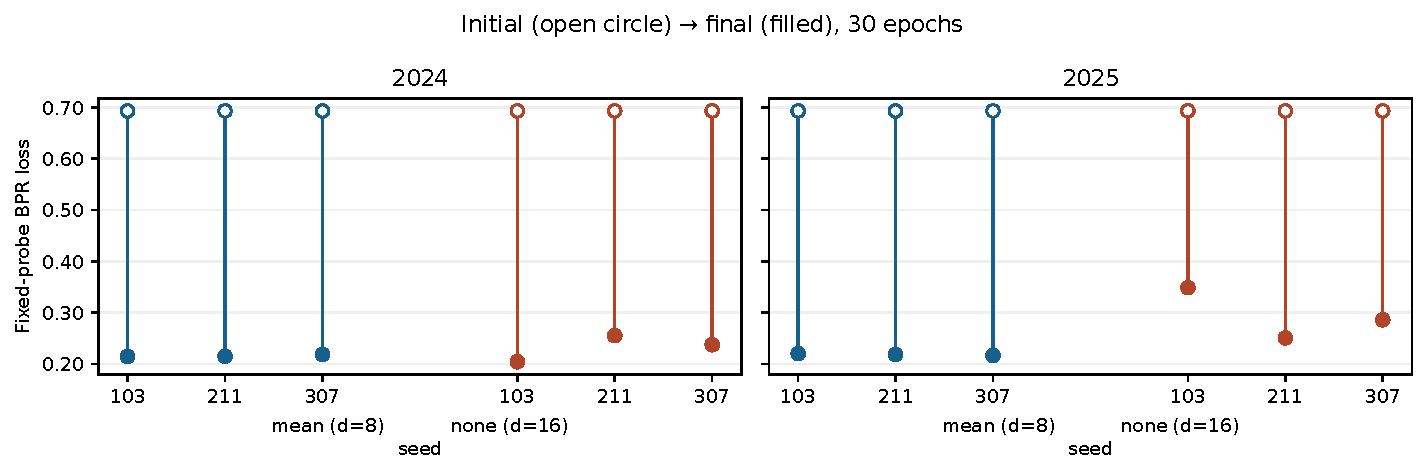
\includegraphics[width=\linewidth]{figures/q2_maude_learning_en.pdf}
\caption{MAUDE Q2: before/after losses on the fixed learning probe for the 12 selected GraphSAGE refits (\emph{mean}/\emph{none}, 2024/2025 tests, three seeds each). These are two probe measurements, before and after training, not per-epoch loss trajectories.}
\label{fig:q2-maude-learning}
\end{figure}

\begin{figure}[!htbp]\centering
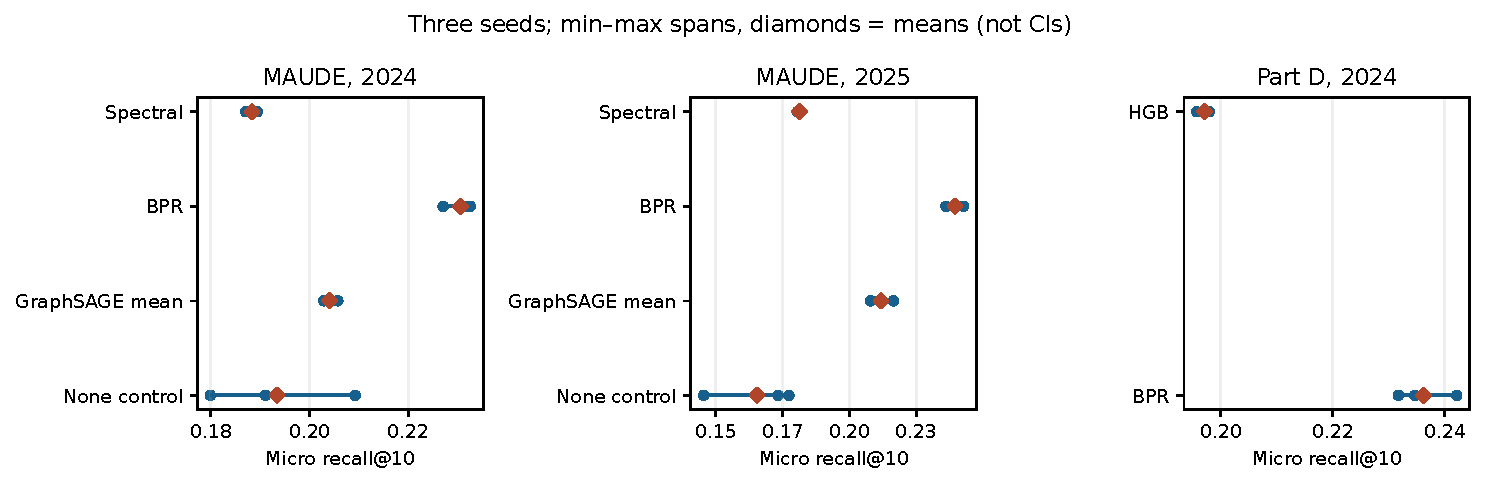
\includegraphics[width=\linewidth]{figures/q2_seed_sensitivity_en.pdf}
\caption{Three-seed points and minimum--maximum ranges for micro recall@10 on MAUDE 2024--2025 and Part D 2024; no bar represents a confidence interval or bootstrap.}
\label{fig:q2-seed-sensitivity}
\end{figure}

No new confidence interval, significance test, or bootstrap accompanies the Q2 tables and figures. The three seeds describe training sensitivity, but their ranges are not intervals for sampling, selection, or training uncertainty. Resource measurements are not comparable as equal budgets: phases share the machine, and dimensions, repetitions, and required time vary.

\par\Needspace{12\baselineskip}
\section{Sealed Part D forecast and future availability}
\label{supp:q2-prospective}

\textbf{Forecast target.} The Q2 protocol defines a forecast of a new relationship observed in the next official annual Part D release, not a clinical prediction for service year 2025 or of a first prescription. The sealed origin is a contemporaneous public capture of the inputs actually used; it does not reconstruct their availability during service years 2019--2024 and will not be recreated when the target is published\cite{hgbq2forecast}.

Run \src{partd-prospective-001} fully recaptured, without authentication, the six public CSVs for 2019--2024: 22,609,355,460 bytes in total, with recorded SHA-256 fingerprints matching the retained local files. The origin was sealed on 3 October 2026 at 22:10:50.231060 UTC; the final forecast was sealed at 22:28:54.610343 UTC. The origin record has SHA-256 \src{ff6641fd17742aad670ed41748cd104e3bed058a65348459c390a716bda44fe3}; the forecast has SHA-256 \src{382e111529f4009c0790267d1518dab050f66d72badc2cb28c8acf2bc120ff9e}. Catalog bodies captured before the fits, after recapture, and before sealing listed no official service-year 2025 node.

The deterministic cohort contains 2,000 NPIs present in the pre-target history. It excludes the union of 2,518 NPIs in the development populations and the 2,288 NPIs in the new Part D comparison, already included in that union. The selection and hashing procedure are sealed without examining target drugs, claims, or labels. Configurations from 2023 validation in the comparison are reused without retuning or seed selection. Seven learned fits and two heuristics each produce 2,112,688 candidate scores; all three seeds are used for HGB because its training set has 359,300 rows, strictly above the 200,000 threshold. All 19 of 19 phases completed (observed wall time 2,241.490 s, maximum aggregate RSS 834,887,680 bytes). No 2025 target label or test metric appears in this forecast.

After exclusions, the pool of NPIs appearing before the target contains 1,490,683 identifiers.
The 2,000 identifiers are selected in hexadecimal order of \texttt{SHA256(salt + NUL + NPI)}, then by NPI, using salt \texttt{q2-prospective-20261003}; the SHA-256 of the sealed list is \src{2ec15e00cb4e90a390b6f668a0637cf250953ceb1ee7adb40334f7e626790319}.
The candidate vocabulary remains that already observed in the 2019--2024 history; the forecast concerns a new relationship in the published files, absent from the provider's history, not a first clinical prescription or a new drug.

Disjoint NPIs do not guarantee statistical independence of observations: drugs, specialties, and network dependencies may be shared. The forecast applies a fixed procedure with refitting on the new cohort's pre-target history only; it is not transfer of an old checkpoint without adaptation.

Fingerprints of the sealed records, including those of the nine score files and seven learned checkpoints, were anchored in public GitHub commit \href{https://github.com/carabistouflette/HealthGraphBench/commit/2a59324003fe8b9c89a5f1e9ff6464f2a76f6ab2}{\nolinkurl{2a59324003fe8b9c89a5f1e9ff6464f2a76f6ab2}}. Public visibility of the repository was observed; the GitHub commit timestamp alone is not treated as proof of visibility. After this anchor, a new public catalog captured on 3 October at 22:43:54.412446 UTC still did not list the 2025 annual node. This capture attests only to the observed state of that catalog at that time, not the absence of private data or all other copies.
The post-anchor catalog response is archived with its exact body: HTTP 200, 278,033 bytes, SHA-256 \src{1388b6cd63fd11d2977cb041d7ade58075b34ef3943253129b1df696325d85fa}; this finding attests only to the timestamped public request.

\textbf{Evaluation status.} The result remains \texttt{sealed\_awaiting\_official\_target\_publication}. The official annual 2025 source, its labels, and a target metric do not exist in the captured evidence; independent evaluation has not passed. The human attestation of non-consultation remains \texttt{unknown}. Sealing and anchoring the scores replace neither the target source nor human attestations; no new origin is assigned to the service year.

\subsection{Conditions for a deferred evaluation}

A later evaluation can begin only after the official annual 2025 node and its primary media are observed in the catalog. The identifier must denote the annual 2025 node, not the shared taxonomy term. Media metadata must establish an exact size and SHA-1 match with the CSV exposed by the primary media; the bytes must then be recaptured publicly and checked against the local target file and its SHA-256. An HTTP, Drupal, modification, republication, or service-year date does not prove historical availability of identical bytes. Labels are evaluated only with the scores already sealed, without retraining, retuning, or seed selection; required non-consultation conditions and human attestations must actually be provided. The future publication date is unknown, and the sealed origin is not moved to that date.

The sealed records and score fingerprints are included under \src{data/q2/}; the nine complete score streams remain in the separate prospective archive. Capture provenance is recorded in \src{q2_partd_prospective_20261003.json}, \src{q2_partd_prospective_publication_20261003.json}, and \src{q2_partd_prospective_publication_catalog_20261003.json}. The post-publication check retains the exact catalog body; it does not turn an observed absence into general proof of absence.

\par\Needspace{12\baselineskip}
\section{Part D API migration and technical reuse}
\label{supp:q2-reuse}

The migration replaces the old active model-gate ranking-reading paths with an API that can load a task, read its strictly prior history, actually run \texttt{fit\_predict}, produce scores, and recompute metrics through \texttt{PartDTask.evaluate}. \texttt{PartDTask.from\_model\_gate} and \texttt{load\_task(..., model\_gate\_dir=...)} are no longer active APIs. Replay examples retained in the README are historical; they do not describe this new interface. Through \texttt{PartDHistoryView}, the API exposes historical drugs/providers, recent specialties, candidates, and support, without target labels; the scorer must return a finite score for every candidate without modifying the list\cite{hgbq2methods}.

The new \texttt{NeighborCosineTop50} model is implemented outside the package. It fits a binary provider--generic-name incidence matrix, computes cosine similarity, retains at most 50 neighbors per provider while excluding the provider itself, and breaks ties by NPI. The score sums similarities of neighbors who have observed the candidate drug. No parameter, seed, or target label is selected; this is an unsupervised fit, so no optimizer loss is invented. Fits at the 2023 and 2024 cutoffs save NPZ checkpoints; after reloading, score identity is checked on control lists of 1,004 and 1,038 candidates, respectively, not by a new full scoring pass.

\begin{table}[!htbp]\centering\small
\caption{Raw--fit--score--evaluation reuse demonstration: the external cosine model is untuned; the SDK logistic model retains the historical 18-epoch algorithm and is not the Q2 grid's LBFGS winner.}
\label{tab:q2-reuse}
% Derived from completed Q2 JSON; no new numerical experiment.
\begin{tabularx}{\linewidth}{@{}Xrr@{}}
\toprule
Method & Val. 2023 & Test 2024 \\
\midrule
Out-of-package cosine top50 & $0.260960$ & $0.258583$ \\
SDK logistic (18 epochs) & $0.178460$ & $0.168188$ \\
\bottomrule
\end{tabularx}

\end{table}

The workflow was run in a wheel built from a clean clone at commit \src{f8ea41c4d8f090560fbdbc698db2300821b9cfef}; the version 0.2.0 development wheel has SHA-256 \src{b5c776556ef64686804c4dec6e354127c59c3db441710519da793ffee6117428}. The isolated driver uses \texttt{python -I} from its phase, the 40 verified package files in \texttt{site-packages}, and no editable environment, \texttt{PYTHONPATH}, or whitelist patch. All six CSVs were verified, fresh preparation was produced, cosine and the genuine public logistic model were fitted, all candidates were scored, and evaluation was recomputed. In the 2024 test, 981 of 2,000 providers have no positive; they remain included in the workload. The 18-epoch SDK logistic model is not the logistic LBFGS comparator selected on validation in the Part D Q2 grid; these results demonstrate technical reuse, not an additional tuned comparison.

Reconstruction commands run in a clone of the original repository, not from vendored read-only files. The provenance commit for the RC3 snapshot is \src{6b4ae00ebc4b701d757260616ccb0df16f51467b}; each published run also retains its own executed-code commit (S12). Supply user-provided raw files matching the manifests, verify their fingerprints, copy the exact protocol included under \src{data/q2/}, and choose a new output directory. The compact package does not contain the full raw streams. Example clone and variables to adapt to the files actually acquired:

\begin{Verbatim}[fontsize=\footnotesize]
git clone https://github.com/carabistouflette/HealthGraphBench.git q2-original
git -C q2-original checkout 6b4ae00ebc4b701d757260616ccb0df16f51467b
cd q2-original
Q2_PROTOCOL=/path/to/HealthGraphBench_RC3/data/q2/q2_scientific_protocol_20261003.json
Q2_PROTOCOL_SHA256=22b3b308e1ddd55f9ebfc388edc1a08ba3dc8a4a83205b230406643155536db7
python scripts/run_q2_maude.py --source-root "$MAUDE_RAW" \
  --protocol "$Q2_PROTOCOL" --protocol-sha256 "$Q2_PROTOCOL_SHA256" \
  --output-dir NEW/maude
python scripts/run_q2_cms.py --source-root "$CMS_RAW" \
  --protocol "$Q2_PROTOCOL" --protocol-sha256 "$Q2_PROTOCOL_SHA256" \
  --output-dir NEW/cms
python scripts/run_q2_partd.py --source-root "$PARTD_RAW" \
  --protocol "$Q2_PROTOCOL" --protocol-sha256 "$Q2_PROTOCOL_SHA256" \
  --output-dir NEW/partd
\end{Verbatim}

MAUDE completion is a separate path that requires the archived complete validation and the same raw root, not a new grid:

\begin{Verbatim}[fontsize=\footnotesize]
python scripts/run_q2_maude.py --complete-validation ROOT001 \
  --source-root "$MAUDE_RAW" --protocol "$Q2_PROTOCOL" \
  --protocol-sha256 "$Q2_PROTOCOL_SHA256" --output-dir NEW/maude-completion
\end{Verbatim}

The original forecast calculation used the completed Part D comparison and raw CSVs. The command below documents that path: a new run would have a new origin and would not replace the sealed scores. Deferred evaluation must use the original retained outputs, without refitting:

\begin{Verbatim}[fontsize=\footnotesize]
python scripts/run_q2_prospective_partd.py forecast \
  --source-root "$PARTD_RAW" --comparison-dir "$PARTD_COMPARISON" \
  --protocol "$Q2_PROTOCOL" --protocol-sha256 "$Q2_PROTOCOL_SHA256" \
  --output-dir NEW/partd-prospective
\end{Verbatim}
For the raw--wheel reuse demonstration, also use an interpreter from the verified clean wheel and a new destination:

\begin{Verbatim}[fontsize=\footnotesize]
python scripts/run_q2_reuse.py --source-root "$PARTD_RAW" \
  --protocol "$Q2_PROTOCOL" --protocol-sha256 "$Q2_PROTOCOL_SHA256" \
  --output-dir NEW/reuse --reuse-python "$REUSE_PYTHON"
\end{Verbatim}

The experiment archives remain separate from the compact manuscript ZIP: MAUDE 141,798,509 bytes (SHA-256 \src{dbce2d88f335b0b718d2decc750dae2638f6de877e8542fb93857a6691a0d637}), CMS 4,569,115 bytes (\src{a11d34e9946c6c03b4b092a423d421094b808db8067ab30777eb2f6b1751cb80}), Part D 630,693,314 bytes (\src{abaf9d40356dc6a8dc02cdddc5fa70328f9e18d082f7f2fabc0989328de3fca4}), reuse 13,086,403 bytes (\src{b0b2cddc54be88120dc6933f544cfa5d4be3811b77d1b65bb15a5e403c66315a}), and prospective forecast 115,004,400 bytes (\src{ced58e93d6168e6767bbbf34d6eb9a5785b4e8279ea59f012749c1aba474d35c}). The MAUDE/CMS/Part D/reuse/forecast archives do not include raw sources; the compact RC3 package therefore does not claim to contain the 193 comparison-fit checkpoints, the nine complete prospective score files, or the full Q2 streams. These artifacts remain in external archives indexed by their ledgers and fingerprints; users must provide the true raw data from the prescribed sources and verify them before execution.

Verification reports are referenced in \src{data/q2/q2_runtime_verification_20261003.json} and \src{data/q2/q2_prospective_software_preflight_20261003.json}. The former records 80 software tests with no failures; wheel-loading checks and controller preflight remain software evidence, not external scientific validation. The prospective preflight uses 4,000 synthetic identifiers and fictitious drugs; its recall@10 = 0.5 and @20 = 1.0 demonstrate only the computation path on a fixture. They are neither a medical source nor a health-model result. The effective reuse run was performed by an assistant/agent: no study with an external human participant was conducted, and this gate remains pending. Author names, affiliations, declarations, and human approvals remain to be established separately.
